\documentclass{beamer}
\usetheme{Boadilla}
\usepackage[utf8]{inputenc}
\usepackage{helvet}
\usepackage[english, ngerman]{babel}

\usepackage{natbib} % for the bibliography
\bibliographystyle{plainnat}
\setcitestyle{numbers}

\usecolortheme{tum}
\useoutertheme{tum}

\setbeamerfont{author}{size=\footnotesize}
\setbeamerfont{date}{size=\scriptsize}
\setbeamerfont{date}{size=\scriptsize}

\useinnertheme{rectangles}

\usepackage{pgf}  
\usepackage{tikz}
\logo{\pgfputat{\pgfxy(-0.2, 8.5)}{\pgfbox[right,top]{
\begin{tikzpicture}[y=0.38pt, x=0.38pt,yscale=-1, inner sep=0pt, outer sep=0pt]
\begin{scope}[cm={{1.25,0.0,0.0,-1.25,(0.0,35.4325)}}]
    \path[fill=tum,nonzero rule] (4.8090,23.2950) -- (4.8090,-0.0020) --
      (9.8590,-0.0020) -- (9.8590,23.2600) -- (15.4730,23.2600) -- (15.4730,-0.0020)
      -- (31.5390,-0.0020) -- (31.5390,23.0140) -- (37.2580,23.0140) --
      (37.2580,0.0060) -- (42.5550,0.0060) -- (42.5550,23.0140) -- (48.3440,23.0140)
      -- (48.3440,0.0060) -- (53.6410,0.0060) -- (53.6410,28.3460) --
      (26.4530,28.3460) -- (26.4530,5.1580) -- (20.6290,5.1580) -- (20.6290,28.3110)
      -- (-0.0000,28.3110) -- (-0.0000,23.2950) -- (4.8090,23.2950) -- cycle;
\end{scope}
\end{tikzpicture}
}}}

\setbeamertemplate{title page}
{
	\vbox{}
	\vfill
	\begin{flushleft}
		\begin{beamercolorbox}[sep=8pt,left]{title}
			\usebeamerfont{title}\inserttitle\par%
			\ifx\insertsubtitle\@empty%
			\else%
				\vskip0.25em%
				{\usebeamerfont{subtitle}\usebeamercolor[fg]{subtitle}\insertsubtitle\par}%
			\fi%
    	\end{beamercolorbox}%
    	\vskip1em\par
		\begin{beamercolorbox}[sep=8pt,left]{author}
		\usebeamerfont{author}\insertauthor
		\end{beamercolorbox}
		\begin{beamercolorbox}[sep=8pt,left]{institute}
		\usebeamerfont{institute}\insertinstitute
		\end{beamercolorbox}
		\begin{beamercolorbox}[sep=8pt,left]{date}
		\usebeamerfont{date}\insertdate
		\end{beamercolorbox}\vskip0.5em
		{\usebeamercolor[fg]{titlegraphic}\inserttitlegraphic\par}
	\end{flushleft}
	\vfill
}

\mode<presentation>

\title{Source Terms}
% \subtitle{Source Terms}

\author{Matilde Tozzi}
\institute[]{Seminar Course - Fundamentals of Wave Simulation - Solving Hyperbolic Systems of PDEs}
\date[January 2024]{January 2024}

\renewcommand{\emph}[1]{\textcolor{tum}{\textbf{#1}}}

\begin{document}
\beamertemplatenavigationsymbolsempty

\begin{frame}
	\titlepage
\end{frame}

% 2. Slide: TOC
\begin{frame}
	\frametitle{Table of contents}
	\tableofcontents
\end{frame}


%%%%%%%%%%%%%%%%%%% From Conservation Laws to Balance Laws
\section{From Conservation Laws to Balance Laws}
\begin{frame}
	\frametitle{From Conservation Laws to Balance Laws}
	Our reference equation is
	\begin{equation}
		q_t +f(q)_x = \psi(q)
	\end{equation}
	where
	\begin{itemize}
		\item the homogeneous equation $q_t +f(q)_x = 0$ is \emph{hyperbolic}
		\item $\psi(q)$ (the \emph{source terms}) don't depend on derivatives of $q$
		      \begin{itemize}
			      \item $\Rightarrow$ $q_t = \psi(q)$ is an independent system of ODEs
		      \end{itemize}
	\end{itemize}
\end{frame}



%%%%%%%%%%%%%%%%%%% The Advection-Reaction Equation
\section{The Advection-Reaction Equation}


















%%%%%%%%%%%%%%%%%%% Godunov-Strang splitting
\section{Godunov-Strang splitting}
%%%%%%%%%%%%%%%%%%% The Unsplit Method
\subsection{The Unsplit Method}















%%%%%%%%%%%%%%%%%%% Godunov Splitting
\subsection{Godunov Splitting}














%%%%%%%%%%%%%%%%%%% General Formulation
\subsection{General Formulation}

















%%%%%%%%%%%%%%%%%%% Strang Splitting
\subsection{Strang Splitting}





















%%%%%%%%%%%%%%%%%%% Accuracy
\subsection{Accuracy}
















%%%%%%%%%%%%%%%%%%% Implicit Methods and Choice of ODE Solver
\section{Implicit Methods and Choice of ODE Solver}















%%%%%%%%%%%%%%%%%%% Stiff and Singular Source Terms and the Associated Numerical Difficulties
\section{Stiff and Singular Source Terms and the Associated Numerical Difficulties}
asdf



































% \begin{frame}
% 	\frametitle{Frametitle}
% 	\framesubtitle{Framesubtitle}
% 	Lorem ipsum
% 	\begin{itemize}
% 		\item Item 1
% 		\item Item 2
% 		\item Item 3
% 	\end{itemize}
% 	\vfill
% 	Question?
% 	\begin{columns}[t]
% 		\column{.45\textwidth}
% 		\begin{block}{Block 1}
% 			Text 1
% 		\end{block}
% 		\column{.45\textwidth}
% 		\begin{block}{Block 2}
% 			Text 2
% 		\end{block}
% 	\end{columns}
% \end{frame}



% % Further Slides
% \section{Titles}
% \begin{frame}
% 	\frametitle{Title}
% 	Each frame should have a title.
% \end{frame}



% \subsection{Subsection no.1.1  }
% \begin{frame}
% 	Without title something is missing.
% \end{frame}



% \section{Lists}
% \subsection{Lists I}
% \begin{frame}
% 	\frametitle{Unnumbered Lists}
% 	\begin{itemize}
% 		\item Introduction to  \LaTeX
% 		\item Second bullet point
% 		\item And a third one
% 		\item The last one
% 	\end{itemize}
% \end{frame}



% \begin{frame}\frametitle{Lists with Pause}
% 	\begin{itemize}
% 		\item Introduction to  \LaTeX \pause
% 		\item Second bullet point \pause
% 		\item And a third one \pause
% 		\item The last one
% 	\end{itemize}
% \end{frame}



% \subsection{Lists II}
% \begin{frame}
% 	\frametitle{Numbered Lists}
% 	\begin{enumerate}
% 		\item Introduction to  \LaTeX
% 		\item Second bullet point
% 		\item And a third one
% 		\item The last one
% 	\end{enumerate}
% \end{frame}



% \begin{frame}
% 	\frametitle{Numbered Lists with Pause}
% 	\begin{enumerate}
% 		\item Introduction to  \LaTeX \pause
% 		\item Second bullet point \pause
% 		\item And a third one \pause
% 		\item The last one
% 	\end{enumerate}
% \end{frame}



% \section{Tables}
% \subsection{Tables}
% \begin{frame}
% 	\frametitle{Tables}
% 	\begin{tabular}{|c|c|c|}
% 		\hline
% 		\textbf{Title} & \textbf{Title} & \textbf{Title} \\
% 		\hline
% 		First column   & Second column  & \LaTeX         \\
% 		\hline
% 		Second row     & \LaTeX         & Last column    \\
% 		\hline
% 	\end{tabular}
% \end{frame}



% \section{Blocks \& Math}
% \subsection{Blocks}
% \begin{frame}
% 	\frametitle{Blocks}

% 	\begin{block}{This is a simple block}
% 		It should contain some text.
% 	\end{block}

% 	\begin{exampleblock}{Example Block}
% 		This may be an example.
% 	\end{exampleblock}


% 	\begin{alertblock}{Warning}
% 		The violent color indicates that this block may alert of something.
% 	\end{alertblock}
% \end{frame}



% \subsection{Math}
% \begin{frame}
% 	\frametitle{Math Expressions are a Breeze with \LaTeX \ldots}

% 	\begin{equation}
% 		p(\mathbf{x}_{k}|\mathbf{Z}_{k}) = \frac{p(\mathbf{z}_{k}|\mathbf{x     }_{k})p(\mathbf{x}_{k}|\mathbf{Z}_{k-1})}{\int \! p(\mathbf{z}_{k}|\mathbf{     x}_{k})p(\mathbf{x}_{k}|\mathbf{Z}_{k-1})\,d\mathbf{x}_{k}}
% 	\end{equation}

% 	\begin{equation}
% 		w_{k}^{i} \sim w_{k-1}^{i}\frac{p(\mathbf{z}_{k}|\mathbf{x}_{k}^{i})p(\mathbf{x}_{k}^{i}|\mathbf{x}_{k-1}^{i})}{q(\mathbf{x}_{k}^{i}|\mathbf{x}_{k-1}^{i},\mathbf{z}_{k})}
% 	\end{equation}

% 	\ldots and Bayes filtering is great!

% \end{frame}

% \section{Multimedia}
% \subsection{Split Screen}
% \begin{frame}
% 	\frametitle{Splitting Screen}
% 	\begin{columns}

% 		\begin{column}{5cm}
% 			\begin{itemize}
% 				\item Here
% 				\item is some
% 				\item text
% 			\end{itemize}
% 		\end{column}

% 		\begin{column}{5cm}
% 			\begin{tabular}{|c|c|}
% 				\hline
% 				\textbf{On the} & \textbf{other side} \\
% 				\hline
% 				there may       & be a table          \\
% 				\hline
% 				or even         & a picture as        \\
% 				\hline
% 				shown on the    & next frame          \\
% 				\hline
% 			\end{tabular}
% 		\end{column}

% 	\end{columns}
% \end{frame}



% \subsection{Pictures}
% \begin{frame}
% 	\frametitle{Pictures in Latex Beamer Class}
% 	\begin{figure}
% 		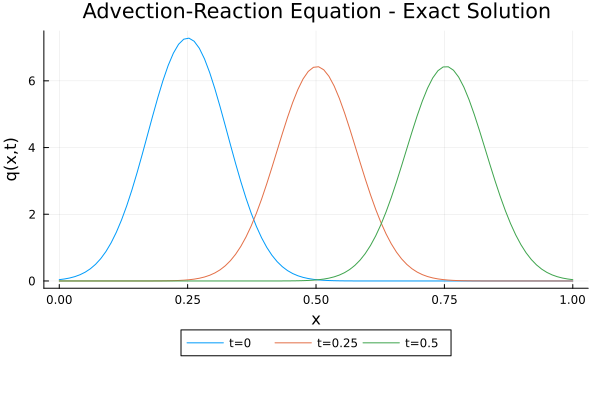
\includegraphics[width=0.5\textwidth]{../Advection.png}
% 		\caption{This is a picture!}
% 	\end{figure}
% \end{frame}



% \subsection{Pictures which Need More Space}
% \begin{frame}[plain]
% 	\frametitle{Plain, or a Way to Get More Space}
% 	\begin{figure}
% 		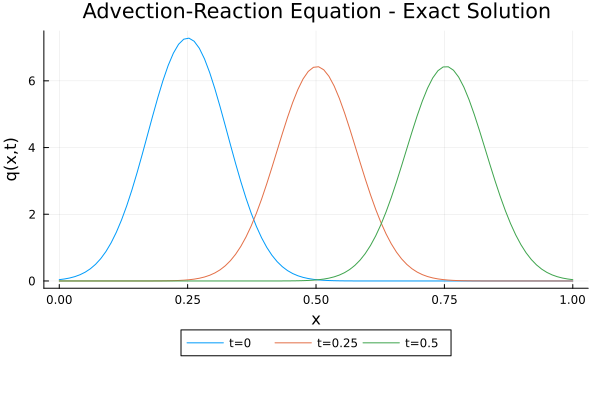
\includegraphics[width=0.5\textwidth]{../Advection.png}
% 		\caption{Picture again.}
% 	\end{figure}
% \end{frame}


\end{document}